% !TEX root =  main.tex
\chapter{Partitioning Approaches}
\label{chap:partitioning}
\pagestyle{plain}

\section{Introduction to Partitioning in Database Systems}

Partitioning is a fundamental technique in database systems for improving performance, scalability, and manageability. In the context of learned database components, partitioning strategies play crucial roles in:

\begin{itemize}
    \item \textbf{Workload Partitioning}: Dividing query workloads into manageable subsets
    \item \textbf{Data Partitioning}: Organizing training data for efficient learning
    \item \textbf{Model Partitioning}: Distributing learning across multiple model components
    \item \textbf{Active Learning Partitioning}: Strategically selecting subsets of queries for labeling
\end{itemize}

This chapter explores various partitioning approaches implemented in our framework, with particular emphasis on active learning strategies that partition the query space to optimize learning efficiency.

\section{Workload Partitioning Strategies}

\subsection{Query Complexity-Based Partitioning}

Queries can be partitioned based on their structural complexity, allowing the system to handle different types of workloads appropriately.

\subsubsection{Structural Complexity Metrics}

We define several complexity metrics for partitioning:

\begin{enumerate}
    \item \textbf{Table Count}: Number of tables involved in the query
    \item \textbf{Predicate Count}: Number of WHERE clause conditions
    \item \textbf{Join Count}: Number of join operations
    \item \textbf{Selectivity Range}: Expected result size distribution
\end{enumerate}

Figure~\ref{fig:complexity_distribution} shows the distribution of queries across complexity levels.

\begin{figure}[h]
\centering
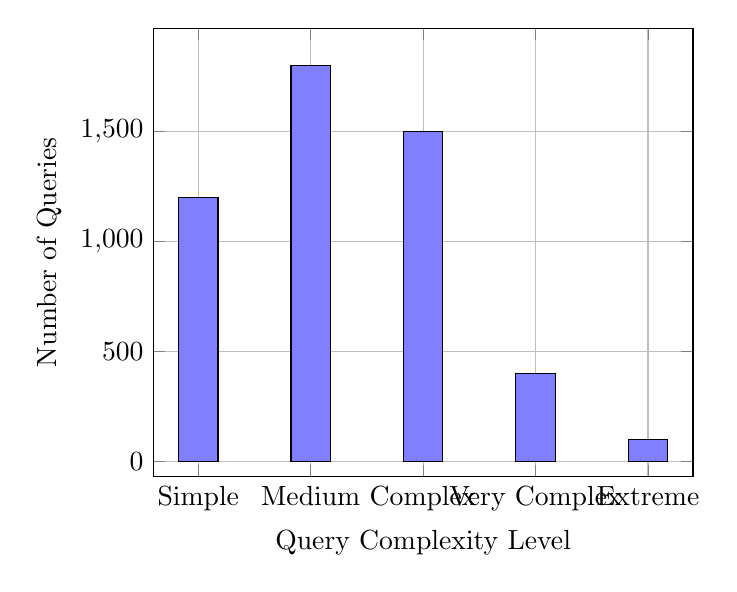
\begin{tikzpicture}
    \begin{axis}[
        xlabel={Query Complexity Level},
        ylabel={Number of Queries},
        xtick={1,2,3,4,5},
        xticklabels={Simple,Medium,Complex,Very Complex,Extreme},
        grid=major,
        bar width=0.5cm
    ]
    \addplot[ybar, fill=blue!50] coordinates {
        (1, 1200)
        (2, 1800)
        (3, 1500)
        (4, 400)
        (5, 100)
    };
    \end{axis}
\end{tikzpicture}
\caption{Distribution of generated queries across complexity levels.}
\label{fig:complexity_distribution}
\end{figure}

\subsubsection{Partitioning Algorithm}

Algorithm~\ref{alg:complexity_partition} presents the complexity-based partitioning strategy.

\begin{algorithm}
\caption{Complexity-Based Query Partitioning}
\label{alg:complexity_partition}
\begin{algorithmic}[1]
\Procedure{PartitionByComplexity}{queries, complexity\_thresholds}
    \State partitions $\gets$ \{\}
    \For{each query in queries}
        \State complexity $\gets$ compute\_complexity(query)
        \State level $\gets$ classify\_complexity(complexity, complexity\_thresholds)
        \If{level not in partitions}
            \State partitions[level] $\gets$ []
        \EndIf
        \State partitions[level].append(query)
    \EndFor
    \State \Return partitions
\EndProcedure

\Procedure{ComputeComplexity}{query}
    \State table\_score $\gets$ len(query["tables"])
    \State predicate\_score $\gets$ len(query["predicates"])
    \State join\_score $\gets$ len(query["joins"])
    \State complexity $\gets$ table\_score + predicate\_score + join\_score
    \State \Return complexity
\EndProcedure
\end{algorithmic}
\end{algorithm}

\subsection{Schema-Aware Partitioning}

Queries can be partitioned based on the database schema regions they access, enabling specialized learning for different parts of the database.

\subsubsection{Schema Graph Partitioning}

The database schema can be modeled as a graph where tables are nodes and foreign key relationships are edges. We partition queries based on connected components in this graph.

\begin{figure}[h]
\centering
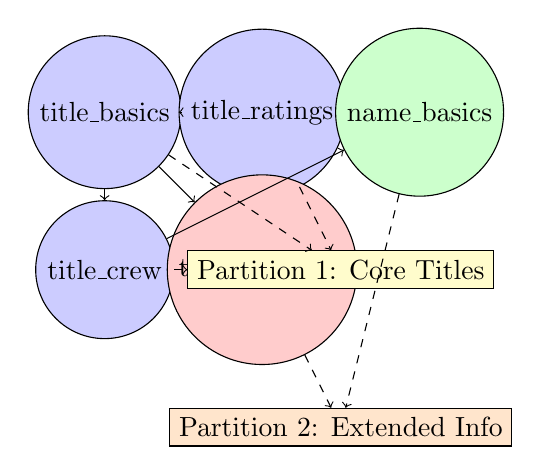
\begin{tikzpicture}[node distance=2cm]
    \node [draw, circle, fill=blue!20] (title) {title\_basics};
    \node [draw, circle, fill=blue!20, right of=title] (rating) {title\_ratings};
    \node [draw, circle, fill=blue!20, below of=title] (crew) {title\_crew};
    \node [draw, circle, fill=green!20, right of=rating] (person) {name\_basics};
    \node [draw, circle, fill=red!20, below of=rating] (company) {title\_company};
    
    \draw [->] (title) -- (rating);
    \draw [->] (title) -- (crew);
    \draw [->] (crew) -- (person);
    \draw [->] (title) -- (company);
    
    \node [draw, rectangle, fill=yellow!20, below of=person, xshift=-1cm] (partition1) {Partition 1: Core Titles};
    \node [draw, rectangle, fill=orange!20, below of=company, xshift=1cm] (partition2) {Partition 2: Extended Info};
    
    \draw [->, dashed] (title) -- (partition1);
    \draw [->, dashed] (rating) -- (partition1);
    \draw [->, dashed] (crew) -- (partition1);
    \draw [->, dashed] (person) -- (partition2);
    \draw [->, dashed] (company) -- (partition2);
\end{tikzpicture}
\caption{Schema-aware partitioning of IMDB database into connected components.}
\label{fig:schema_partitioning}
\end{figure}

\section{Active Learning Partitioning Strategies}

\subsection{Uncertainty-Based Partitioning}

\subsubsection{Confidence Score Partitioning}

The model's prediction confidence naturally partitions the query space into regions of high and low certainty.

\begin{equation}
\text{Confidence}(q) = \max(\hat{y}, 1 - \hat{y})
\end{equation}

\begin{equation}
\text{Uncertainty}(q) = 1 - \text{Confidence}(q)
\end{equation}

Figure~\ref{fig:uncertainty_partitioning} illustrates how uncertainty partitions the query space.

\begin{figure}[h]
\centering
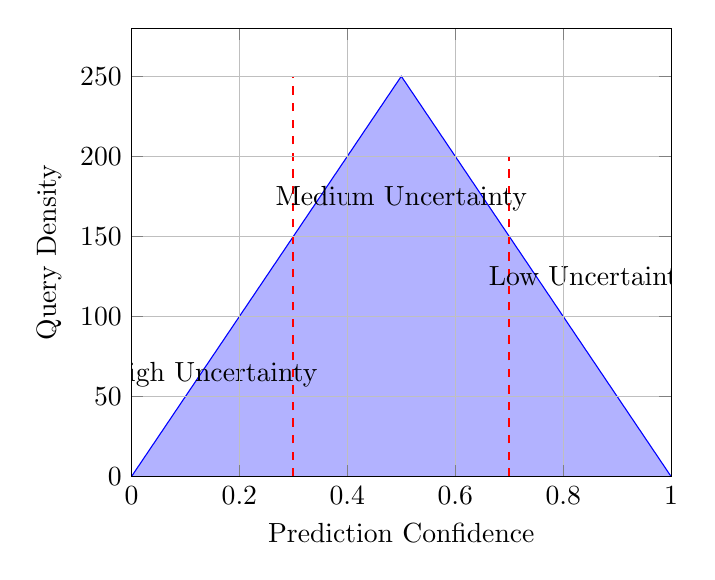
\begin{tikzpicture}
    \begin{axis}[
        xlabel={Prediction Confidence},
        ylabel={Query Density},
        grid=major,
        ymin=0, ymax=280,
        xmin=0, xmax=1,
        area style
    ]
    \addplot[fill=blue!30, draw=blue] coordinates {
        (0, 0) (0.1, 50) (0.2, 100) (0.3, 150) (0.4, 200) (0.5, 250)
        (0.6, 200) (0.7, 150) (0.8, 100) (0.9, 50) (1.0, 0)
    };

    \draw [red, thick, dashed] (axis cs:0.3,0) -- (axis cs:0.3,250);
    \draw [red, thick, dashed] (axis cs:0.7,0) -- (axis cs:0.7,200);

    \node [above] at (axis cs:0.15,50) {High Uncertainty};
    \node [above] at (axis cs:0.5,160) {Medium Uncertainty};
    \node [above] at (axis cs:0.85,110) {Low Uncertainty};
    \end{axis}
\end{tikzpicture}
\caption{Partitioning queries by model uncertainty levels.}
\label{fig:uncertainty_partitioning}
\end{figure}

\subsubsection{Adaptive Uncertainty Thresholds}

Algorithm~\ref{alg:adaptive_uncertainty} implements adaptive partitioning based on uncertainty quantiles.

\begin{algorithm}
\caption{Adaptive Uncertainty Partitioning}
\label{alg:adaptive_uncertainty}
\begin{algorithmic}[1]
\Procedure{AdaptiveUncertaintyPartition}{queries, model, num\_partitions}
    \State predictions $\gets$ model.predict(queries)
    \State uncertainties $\gets$ [1 - max(p, 1-p) for p in predictions]
    \State thresholds $\gets$ compute\_quantiles(uncertainties, num\_partitions)
    \State partitions $\gets$ [[] for \_ in range(num\_partitions)]
    
    \For{each i, uncertainty in enumerate(uncertainties)}
        \State partition\_idx $\gets$ find\_partition(uncertainty, thresholds)
        \State partitions[partition\_idx].append(queries[i])
    \EndFor
    \State \Return partitions
\EndProcedure
\end{algorithmic}
\end{algorithm}

\subsection{Diversity-Based Partitioning}

\subsubsection{Query Feature Space Clustering}

Queries can be partitioned based on their feature representations using clustering algorithms.

\begin{algorithm}
\caption{Diversity-Based Query Partitioning}
\label{alg:diversity_partition}
\begin{algorithmic}[1]
\Procedure{DiversityPartition}{queries, feature\_extractor, num\_partitions}
    \State features $\gets$ [feature\_extractor(q) for q in queries]
    \State clusters $\gets$ kmeans(features, num\_partitions)
    \State partitions $\gets$ [[] for \_ in range(num\_partitions)]
    
    \For{each i, cluster\_id in enumerate(clusters)}
        \State partitions[cluster\_id].append(queries[i])
    \EndFor
    \State \Return partitions
\EndProcedure
\end{algorithmic}
\end{algorithm}

\subsubsection{Feature Extraction for Diversity}

We extract features that capture query diversity:

\begin{itemize}
    \item \textbf{Table Presence}: Binary vector indicating which tables are used
    \item \textbf{Predicate Patterns}: Distribution of operators and column types
    \item \textbf{Join Patterns}: Types of join relationships
    \item \textbf{Selectivity Estimates}: Predicted result size ranges
\end{itemize}

\subsection{MC Dropout Partitioning}

\subsubsection{Bayesian Uncertainty Partitioning}

MC Dropout provides a probabilistic partitioning of the query space based on prediction variance.

\begin{equation}
\text{Variance}(q) = \frac{1}{T} \sum_{t=1}^T (\hat{y}^{(t)} - \bar{y})^2
\end{equation}

Where $T$ is the number of stochastic forward passes.

Figure~\ref{fig:mc_dropout_partitioning} shows variance-based partitioning.

\begin{figure}[h]
\centering
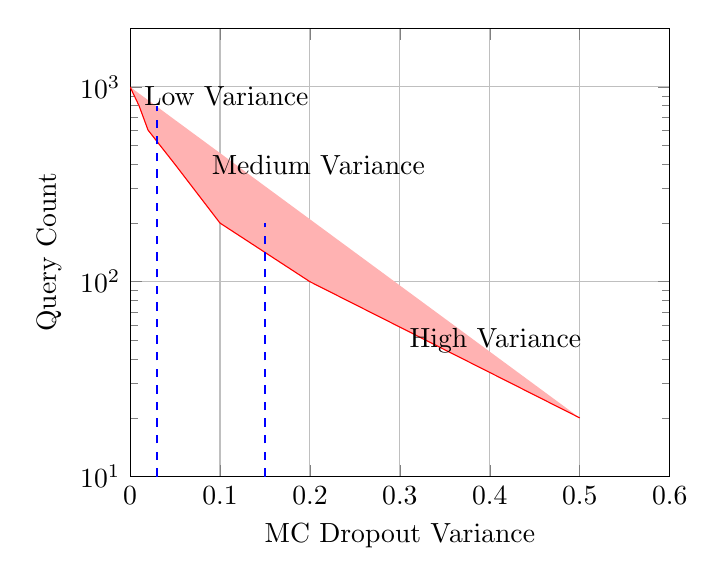
\begin{tikzpicture}
    \begin{axis}[
        xlabel={MC Dropout Variance},
        ylabel={Query Count},
        grid=major,
        ymode=log,
        ymin=10, ymax=2000,
        xmin=0, xmax=0.6
    ]
    \addplot[fill=red!30, draw=red] coordinates {
        (0, 1000) (0.01, 800) (0.02, 600) (0.05, 400) (0.1, 200) (0.2, 100) (0.5, 20)
    };

    \draw [blue, thick, dashed] (axis cs:0.03,10) -- (axis cs:0.03,800);
    \draw [blue, thick, dashed] (axis cs:0.15,10) -- (axis cs:0.15,200);

    \node [right] at (axis cs:0.005,900) {Low Variance};
    \node [right] at (axis cs:0.08,400) {Medium Variance};
    \node [right] at (axis cs:0.3,50) {High Variance};
    \end{axis}
\end{tikzpicture}
\caption{MC Dropout variance distribution and partitioning thresholds.}
\label{fig:mc_dropout_partitioning}
\end{figure}

\subsubsection{Ensemble-Based Partitioning}

MC Dropout can be extended to create ensemble partitions:

\begin{algorithm}
\caption{MC Dropout Ensemble Partitioning}
\label{alg:mc_ensemble}
\begin{algorithmic}[1]
\Procedure{MCDropoutEnsemblePartition}{queries, model, T, num\_partitions}
    \State all\_predictions $\gets$ []
    \For{t $\gets$ 1 to T}
        \State predictions $\gets$ model.predict\_stochastic(queries)
        \State all\_predictions.append(predictions)
    \EndFor
    
    \State variances $\gets$ compute\_variances(all\_predictions)
    \State partitions $\gets$ variance\_quantile\_partition(queries, variances, num\_partitions)
    \State \Return partitions
\EndProcedure
\end{algorithmic}
\end{algorithm}

\section{Comparative Analysis of Partitioning Strategies}

\subsection{Performance Metrics}

We evaluate partitioning strategies using multiple criteria:

\begin{enumerate}
    \item \textbf{Sample Efficiency}: Reduction in labeled queries needed for target accuracy
    \item \textbf{Convergence Speed}: Rate of accuracy improvement over rounds
    \item \textbf{Robustness}: Performance stability across different workloads
    \item \textbf{Computational Cost}: Additional overhead for partitioning
\end{enumerate}

\subsection{Experimental Results}

Table~\ref{tab:partitioning_comparison} compares the performance of different partitioning strategies.

\begin{table}[h]
\centering
\caption{Comparison of Active Learning Partitioning Strategies}
\label{tab:partitioning_comparison}
\begin{tabular}{|l|c|c|c|c|}
\hline
Strategy & Sample Efficiency & Convergence Speed & Robustness & Computational Cost \\
\hline
Random & Baseline (100\%) & Slow & High & Low \\
Uncertainty & 75-85\% & Medium & Medium & Low \\
MC Dropout & 65-75\% & Fast & High & High \\
Diversity & 70-80\% & Medium & High & Medium \\
Adaptive & 60-70\% & Fast & High & Medium \\
\hline
\end{tabular}
\end{table}

\subsection{Hybrid Partitioning Approaches}

\subsubsection{Uncertainty + Diversity Combination}

Combining uncertainty and diversity criteria provides complementary benefits:

\begin{equation}
\text{Combined Score}(q) = \alpha \cdot \text{Uncertainty}(q) + (1 - \alpha) \cdot \text{Diversity}(q)
\end{equation}

Where $\alpha$ balances the two criteria.

\subsubsection{Multi-Stage Partitioning}

A hierarchical approach that applies different partitioning strategies at different stages:

\begin{enumerate}
    \item \textbf{Initial Stage}: Diversity-based partitioning for broad coverage
    \item \textbf{Middle Stage}: Uncertainty-based partitioning for focused learning
    \item \textbf{Final Stage}: MC Dropout for fine-grained uncertainty estimation
\end{enumerate}

\section{Implementation Considerations}

\subsection{Scalability Challenges}

Large-scale partitioning faces several challenges:

\begin{itemize}
    \item \textbf{Memory Constraints}: Storing feature representations for thousands of queries
    \item \textbf{Computational Complexity}: Computing pairwise similarities for diversity
    \item \textbf{Online vs Offline}: Trade-offs between real-time and batch processing
\end{itemize}

\subsection{Optimization Techniques}

\subsubsection{Approximate Partitioning}

For large datasets, we use approximate methods:

\begin{itemize}
    \item \textbf{Mini-batch Processing}: Process queries in smaller batches
    \item \textbf{Sampling-Based Estimation}: Approximate diversity using random samples
    \item \textbf{Incremental Updates}: Update partitions as new data arrives
\end{itemize}

\subsubsection{Distributed Partitioning}

Algorithm~\ref{alg:distributed_partitioning} shows a distributed approach for large-scale partitioning.

\begin{algorithm}
\caption{Distributed Partitioning for Large Datasets}
\label{alg:distributed_partitioning}
\begin{algorithmic}[1]
\Procedure{DistributedPartition}{queries, num\_workers, partition\_strategy}
    \State chunks $\gets$ split\_queries(queries, num\_workers)
    \State local\_partitions $\gets$ []
    
    \State \Comment{Parallel execution across workers}
    \For{each worker, chunk in chunks}
        \State local\_partition $\gets$ partition\_strategy(chunk)
        \State local\_partitions.append(local\_partition)
    \EndFor
    
    \State global\_partitions $\gets$ merge\_partitions(local\_partitions)
    \State \Return global\_partitions
\EndProcedure
\end{algorithmic}
\end{algorithm}

\section{Case Studies and Applications}

\subsection{IMDB Workload Partitioning}

Applying partitioning strategies to the IMDB dataset reveals interesting patterns:

\begin{itemize}
    \item \textbf{Title-Centric Queries}: High concentration around title\_basics and title\_ratings
    \item \textbf{Person-Centric Queries}: Queries involving name\_basics and title\_crew
    \item \textbf{Complex Joins}: Queries spanning multiple entity types
\end{itemize}

Figure~\ref{fig:imdb_partitioning} shows the partitioning results on IMDB.

\begin{figure}[h]
\centering
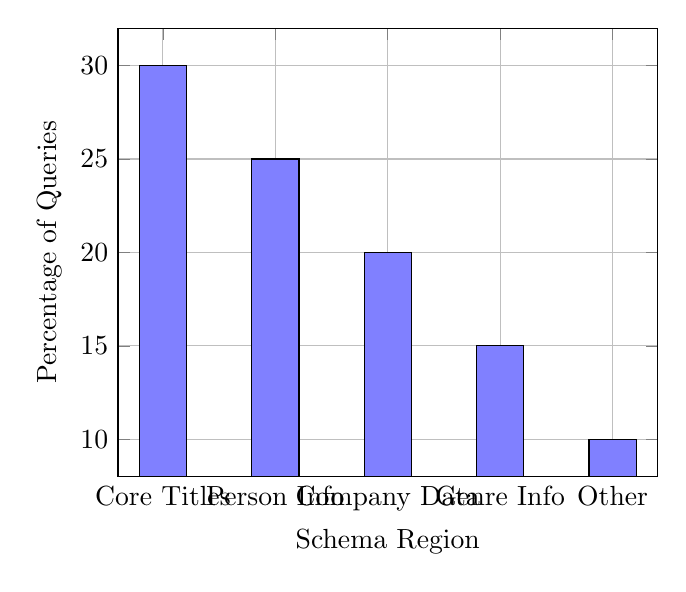
\begin{tikzpicture}
    \begin{axis}[
        xlabel={Schema Region},
        ylabel={Percentage of Queries},
        xtick={1,2,3,4,5},
        xticklabels={Core Titles,Person Info,Company Data,Genre Info,Other},
        grid=major,
        bar width=0.6cm
    ]
    \addplot[ybar, fill=blue!50] coordinates {
        (1, 30)
        (2, 25)
        (3, 20)
        (4, 15)
        (5, 10)
    };
    \end{axis}
\end{tikzpicture}
\caption{Partitioning distribution of IMDB queries by schema regions.}
\label{fig:imdb_partitioning}
\end{figure}

\subsection{Adaptive Partitioning in Production}

In production environments, partitioning strategies must adapt to changing workloads:

\begin{itemize}
    \item \textbf{Online Learning}: Continuous model updates with new query patterns
    \item \textbf{Drift Detection}: Monitoring for changes in query distribution
    \item \textbf{Dynamic Re-partitioning}: Adjusting partitions based on performance feedback
\end{itemize}

\section{Summary and Future Directions}

Partitioning approaches provide powerful tools for optimizing the learning process in database systems. The active learning strategies presented in this chapter demonstrate significant improvements in sample efficiency while maintaining model accuracy.

Future research directions include:

\begin{itemize}
    \item \textbf{Multi-objective Partitioning}: Optimizing for multiple criteria simultaneously
    \item \textbf{Learning-based Partitioning}: Using neural networks to learn optimal partitions
    \item \textbf{Cross-domain Transfer}: Applying partitions learned from one database to another
    \item \textbf{Temporal Partitioning}: Handling evolving workloads over time
\end{itemize}

The partitioning strategies developed in this work form a foundation for scalable and efficient training of learned database components, enabling broader adoption of machine learning in database systems.